% ----------------------------------------------------------
% Coleta e Tratamento dos Dados
% ----------------------------------------------------------
\chapter{Coleta e Tratamento dos Dados}
\label{cap:coleta}
% ----------------------------------------------------------

Este capítulo descreve os aspectos operacionais da arquitetura tecnológica de redes do campus, detalhando as ferramentas e dispositivos que dão suporte à infraestrutura. Adicionalmente, expõe-se o processo de consistência inicial, limpeza e higienização das bases de dados brutas de telemetria por meio da importação do relatório de validação.

\section{Ferramentas e Infraestrutura de Rede}
\label{sec:coleta_ferramentas}

A infraestrutura sob monitoramento é suportada por um conjunto integrado de ferramentas de gerência, segurança e controle operacional.

\subsection{Firewall (pfSense)}
O pfSense atua como o \textit{gateway} principal de borda e servidor de firewall da rede local. Ele é encarregado de realizar o roteamento inter-VLAN, gerenciar servidores DHCP para a distribuição dinâmica de endereços IPs aos dispositivos sem fio, controlar políticas de segurança lógica por meio de tabelas de firewall e atuar como concentrador de tráfego, servindo como o ponto central para monitorar as taxas volumétricas globais direcionadas à Internet.

\subsection{Controladora Ruckus (SmartZone)}
A controladora física Ruckus SmartZone gerencia centralizadamente os Access Points Ruckus distribuídos nos prédios acadêmicos do campus. Ela coordena dinamicamente a potência de transmissão, a seleção de canais de RF e as chaves de criptografia WPA2-Enterprise das redes sem fio institucionais. A SmartZone expõe as estatísticas operacionais dos rádios via SNMP e atua como servidora Syslog, despachando logs detalhados de transições de conexão de clientes.

\subsection{Controladora UniFi (UniFi Controller)}
A controladora baseada em software UniFi Controller é instalada localmente no servidor de gerência para monitorar os rádios Ubiquiti das unidades de pesquisa e escritórios administrativos específicos. O UniFi Controller gerencia as configurações dos APs UniFi e disponibiliza os parâmetros físicos de rádio de cada cliente (como sinal RSSI e CCQ) por meio de um serviço HTTP API local estruturado em formato JSON.

\subsection{Plataforma de Visualização (Grafana)}
O Grafana é empregado nesse trabalho como plataforma de análise de dados operacionais em tempo real e visualização de métricas históricas. Ele consome dados de séries temporais das controladoras para alimentar painéis interativos que monitoram a quantidade de usuários ativos por setor, o consumo agregado de largura de banda e alertas de indisponibilidade de rádios.

Para ilustrar o monitoramento operacional da infraestrutura, a plataforma Grafana foi integrada aos coletores de telemetria, permitindo o acompanhamento em tempo real das conexões ativas e a saúde do espectro. A Figura~\ref{fig:grafana_ruckus_conexoes} ilustra o painel principal de monitoramento de clientes no ecossistema Ruckus, enquanto a Figura~\ref{fig:grafana_unifi_conexoes} apresenta o acompanhamento correspondente na rede UniFi. Os demais painéis operacionais desenvolvidos (incluindo gráficos de desconexões, tráfego por frequência e diagnósticos detalhados por rádio) encontram-se reunidos no Apêndice~\ref{ap:paineis_grafana}.

\begin{figure}[H]
	\centering
	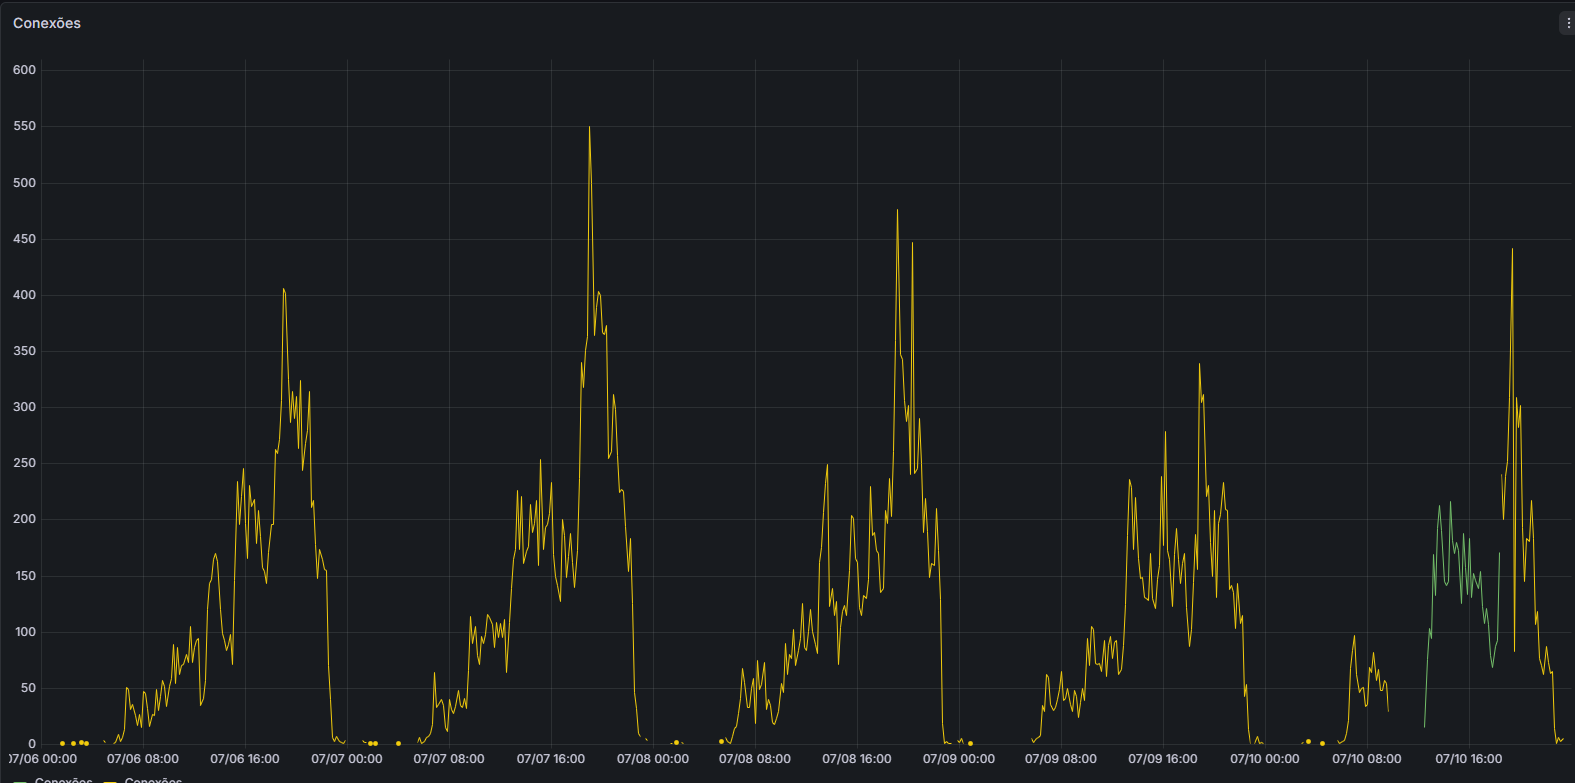
\includegraphics[width=0.85\textwidth]{img/grafana-ruckus-conexoes.png}
	\caption{Painel do Grafana para monitoramento de clientes conectados (Ruckus)}
	\label{fig:grafana_ruckus_conexoes}
	\fonte{Produzido pelos autores (2026).}
\end{figure}

\begin{figure}[H]
	\centering
	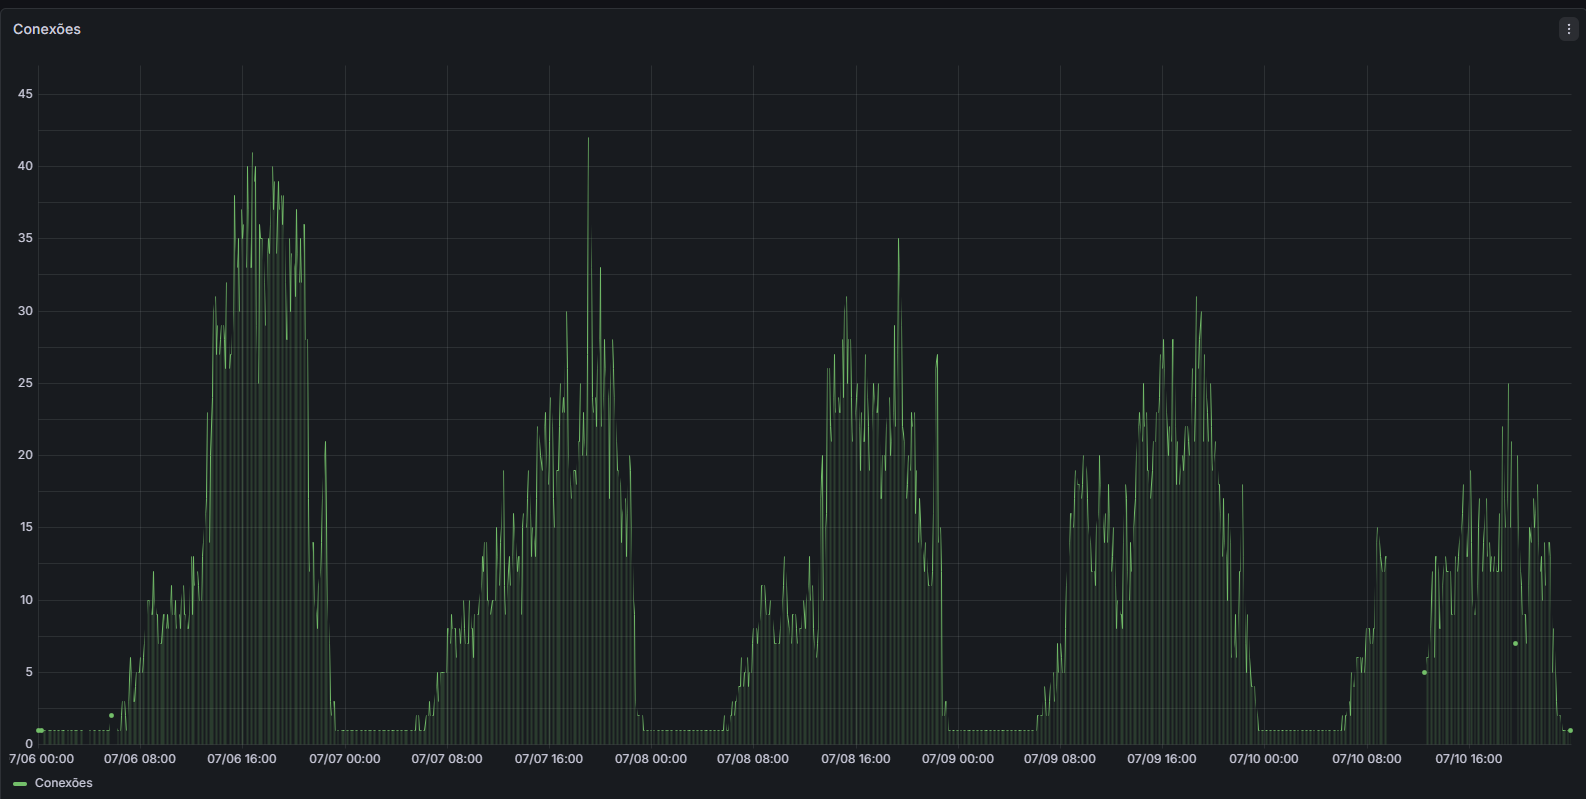
\includegraphics[width=0.85\textwidth]{img/grafana-unifi-conexoes.png}
	\caption{Painel do Grafana para monitoramento de conexões de usuários (UniFi)}
	\label{fig:grafana_unifi_conexoes}
	\fonte{Produzido pelos autores (2026).}
\end{figure}

\subsection{Scripts de Coleta Telemétrica}
Os scripts coletores ativos foram codificados em linguagem Python e agendados para execução periódica no servidor de gerência. Os coletores utilizam a biblioteca \texttt{pysnmp} para interrogar periodicamente as OIDs da Ruckus Wireless e requisições HTTP autenticadas via biblioteca \texttt{requests} para consumir dados em JSON da API UniFi, gravando os logs brutos estruturados diariamente em disco.

\section{Limpeza e Tratamento dos Dados}
\label{sec:coleta_limpeza}

A higienização inicial das informações e a consolidação do conjunto de dados limpo é essencial para eliminar ruídos de polling repetido e valores nulos de conexões inconsistentes. A validação empírica dos dados consolidados é apresentada e discutida a seguir.

\section{Validação de Consistência dos Dados}

\subsection{Quantidade de Registros}

A tabela abaixo resume a quantidade de registros encontrados nos logs de telemetria antes e depois do processo de deduplicação (remoção de duplicados exatos).

\begin{table}[H]
\IBGEtab{%
  \caption{Quantidade de Registros}%
  \label{tab:data_validacao_de_dados_1}%
}{%
  \resizebox{\textwidth}{!}{%
    \begin{tabular}{lcccc}
      \toprule
      Fabricante & Registros Originais & Registros Duplicados Removidos & Registros Limpos & \% de Redundância \\
      \midrule
      \textbf{Ruckus} & 318.074 & 0 & 318.074 & 0,00\% \\
      \textbf{UniFi} & 36.180 & 0 & 36.180 & 0,00\% \\
      \bottomrule
    \end{tabular}%
  }%
}{%
  \fonte{Produzido pelos autores.}%
}
\end{table}

\textit{Nota: Registros duplicados ocorrem por sobreposição em polling repetido do coletor. A remoção evita viés nas análises estatísticas.}

\subsection{Período Coberto pela Coleta}

\begin{table}[H]
\IBGEtab{%
  \caption{Período Coberto pela Coleta}%
  \label{tab:data_validacao_de_dados_2}%
}{%
  \resizebox{\textwidth}{!}{%
    \begin{tabular}{lccc}
      \toprule
      Fabricante & Data/Hora Inicial (Min) & Data/Hora Final (Max) & Duração Efetiva \\
      \midrule
      \textbf{Ruckus} & 23/06/2026 00:00 & 10/07/2026 23:55 & 17 days 23:55:00 \\
      \textbf{UniFi} & 23/06/2026 00:02 & 10/07/2026 23:57 & 17 days 23:55:00 \\
      \bottomrule
    \end{tabular}%
  }%
}{%
  \fonte{Produzido pelos autores.}%
}
\end{table}

\textit{Nota: Ambos os datasets cobrem o mesmo período temporal (de 23/06/2026 00:00 a 10/07/2026 23:55), garantindo que os cenários de carga de rede sejam diretamente comparáveis.}

\subsection{Dados Ausentes (Missing Values)}

O percentual de dados nulos ou ausentes para cada variável após a limpeza:

\begin{table}[H]
\IBGEtab{%
  \caption{Dados Ausentes (Missing Values)}%
  \label{tab:data_validacao_de_dados_3}%
}{%
  \resizebox{\textwidth}{!}{%
    \begin{tabular}{lccc}
      \toprule
      Coluna Padronizada & \% Nulos Ruckus & \% Nulos UniFi & Tipo de Dado \\
      \midrule
      \texttt{timestamp} & 0,00\% & 0,00\% & Datetime \\
      \texttt{AP} & 0,00\% & 0,00\% & Categórico \\
      \texttt{cliente (MAC)} & 0,00\% & 0,00\% & Categórico \\
      \texttt{RSSI} & 10,34\% & 0,00\% & Numérico \\
      \texttt{signal} & 10,34\% & 0,00\% & Numérico \\
      \texttt{noise} & 10,34\% & 0,00\% & Numérico \\
      \texttt{canal} & 0,00\% & 0,00\% & Categórico \\
      \texttt{throughput\_tx\_mbps} & 0,00\% & 0,00\% & Numérico \\
      \texttt{throughput\_rx\_mbps} & 0,00\% & 0,00\% & Numérico \\
      \texttt{link\_speed\_tx\_mbps} & 6,51\% & 0,00\% & Numérico \\
      \texttt{link\_speed\_rx\_mbps} & 100,00\% & 0,00\% & Numérico \\
      \texttt{retransmissoes\_pct} & 0,00\% & 0,00\% & Numérico \\
      \texttt{volume\_tx\_mb} & 0,00\% & 0,00\% & Numérico \\
      \texttt{volume\_rx\_mb} & 0,00\% & 0,00\% & Numérico \\
      \texttt{padrão} & 0,00\% & 0,00\% & Categórico \\
      \bottomrule
    \end{tabular}%
  }%
}{%
  \fonte{Produzido pelos autores.}%
}
\end{table}

\subsection{Tratamento de Valores Nulos}

\begin{itemize}
  \item \textbf{Link Speed no Ruckus}: A taxa de modulação física de TX (\texttt{link\_speed\_tx\_mbps}) foi extraída com sucesso a partir do campo \texttt{throughput\_rate} (em Kbps) nos logs de telemetria da controladora SmartZone. A taxa RX correspondente (\texttt{link\_speed\_rx\_mbps}) não é informada nos logs brutos e é mantida como \texttt{NaN}.
  \item \textbf{Ruído (Noise) e Sinal (Signal) em Ruckus}: Alguns registros continham valores de sinal zerados ou vazios. Onde o sinal era -100 (vazio padrão) e SNR era 0, o ruído foi definido como NaN para evitar distorções de cálculo.
  \item \textbf{Valores Nulos na UniFi}: O dataset UniFi apresenta consistência total (0\% de nulos nas métricas principais de telemetria).

\end{itemize}
\subsection{Padronização das Unidades de Medida}

As colunas foram padronizadas da seguinte forma:
\begin{enumerate}
  \item \textbf{Sinal e Ruído}: Potência medida em \textbf{dBm}.
  \item \textbf{RSSI/SNR}: Medido em \textbf{dB} (ou índice relativo na UniFi).
  \item \textbf{Throughput}: Convertido em \textbf{Mbps} (Megabits por segundo) para Downstream (\texttt{tx}) e Upstream (\texttt{rx}).
  \item \textbf{Volume de Dados}: Convertido em \textbf{MB} (Megabytes) acumulados por cliente no período de observação.
  \item \textbf{Retransmissões}: Medidas em porcentagem (\textbf{\%}) de pacotes retransmitidos.
  \item \textbf{Link Speed}: Modulação de velocidade física convertida em \textbf{Mbps}.

\end{enumerate}
\subsection{Equivalência de Métricas (Mapeamento Ruckus vs UniFi)}

A tabela abaixo mostra a relação entre os campos extraídos de cada fabricante que representam as mesmas grandezas físicas:

\begin{table}[H]
\IBGEtab{%
  \caption{Equivalência de Métricas (Mapeamento Ruckus vs UniFi)}%
  \label{tab:data_validacao_de_dados_4}%
}{%
  \resizebox{\textwidth}{!}{%
    \begin{tabular}{lccc}
      \toprule
      Grandeza Física & Métrica Ruckus (Raw) & Métrica UniFi (Raw) & Coluna Padronizada Final \\
      \midrule
      Potência do Sinal & \texttt{signal\_rssi} & \texttt{signal} & \texttt{signal} (dBm) \\
      Relação Sinal/Ruído & \texttt{snr} & \texttt{rssi} & \texttt{RSSI} (dB) \\
      Throughput Downstream & \texttt{tx\_bytes / uptime} & \texttt{tx\_bytes\_r \textsuperscript{*} 8} & \texttt{throughput\_tx\_mbps} \\
      Throughput Upstream & \texttt{rx\_bytes / uptime} & \texttt{rx\_bytes\_r \textsuperscript{*} 8} & \texttt{throughput\_rx\_mbps} \\
      Retransmissões & \texttt{tx\_retries / (tx\_pkts + tx\_retries)} & \texttt{100 - (ccq / 10)} & \texttt{retransmissoes\_pct} \\
      Volume Trafegado & \texttt{tx\_bytes}, \texttt{rx\_bytes} & \texttt{tx\_bytes\_r \textit{ uptime}, \texttt{rx\_bytes\_r } uptime} & \texttt{volume\_tx\_mb}, \texttt{volume\_rx\_mb} \\
      Modulação de Velocidade & \texttt{throughput\_rate} & \texttt{tx\_rate}, \texttt{rx\_rate} & \texttt{link\_speed\_tx\_mbps}, \texttt{link\_speed\_rx\_mbps} \\
      \bottomrule
    \end{tabular}%
  }%
}{%
  \fonte{Produzido pelos autores.}%
}
\end{table}

